\listfiles
\documentclass[12pt,a4paper]{article}

%% Bibliography style:
\usepackage[pdftex]{graphicx}
\usepackage[compact]{titlesec}
\usepackage{mdwlist}
\usepackage{amsmath}
\usepackage{array}

\usepackage[a4paper,margin=0.97in]{geometry}

\setlength{\parskip}{1.5ex plus 0.5ex minus 0.2ex}
\linespread{1.2}

\title{State Merging for Automatic Test Generation}
\date{}

\author{
Kuan Xiang Wen$^{1}$, Li Xuan Ji$^{1}$, Tan Jiaqi$^{2}$\\
\vspace{1 mm} \\
\small{$^{1}$NUS High School of Math and Science}\\
\small{$^{2}$INFO Division, DSO National Laboratories, Singapore}
}

\newcommand{\klee}{\textsc{klee }}
\newcommand{\leek}{\textsc{leek }}


\begin{document}
%\maketitle
\begin{abstract}
Automatic test generation is the problem of generating test cases in a given program for the purposes of vulnerability detection and program verification. One method of achieving this is Symbolic Execution, which executes the program with \emph{symbolic} variables to quickly test every possible execution path that the program may take. Often symbolic execution creates many execution paths that are similar; our project focuses on determining when these paths can be merged to cut down on repetitive operations. In addition, we have developed a heuristic to avoid merging when the merging algorithm performs worse. We prove our algorithm's soundness and correctness with respect to the base system and demonstrate its practical usefulness by generating test cases for real world programs. We observe speed up from exponential to linear time for certain programs.
\end{abstract}

\section{Introduction}
Today, testing is our first line of defence against software errors. Unfortunately, the only widely used methods to generate test cases are manually writing them and generating them randomly (fuzz testing). Manually writing them is expensive and boring, while generating them randomly has been shown to result in low program coverage. 

Automatic test generation aims to solve this problem by using a computer to generate the test cases for a given program. The main approach to solving it is symbolic execution: instead of running the program on a concrete input, we run it on symbolic input, ie, input that can be 'anything'. When there is a conditional branch in the program, the system follows both branch; on each path it maintains a \emph{path constraint}, constraints that must hold on the input if executing the program on that input causes it to follow that path. On one branch the branch guard is constrained to be true and one where it is false. Because only a small portion of all execution paths are actually possible, a SMT constraint solver is used to check whether a branch condition is provably false; this discards un-executable paths.

The main scalability challenge with symbolic execution is the widely studied \emph{path explosion} problem. The number of execution paths is potentially exponential in the number of branches, leading to too many paths. We have developed an algorithm to determine when certain paths can me merged together, mitigating this problem.

\subsection{Contributions}

In our work, we extend a state-of-the-art symbolic execution engine \klee \cite{klee} which is developed at Stanford Univeristy to handle this problem. \klee is written in C++ and runs on LLVM bitcode. We call our extension \leek. \klee had implemented a function to merge execution states but relied on users to manually annotate the program with merge points. Our contributions are threefold:

\linespread{0}
\begin{enumerate*}

\item We develop an algorithm to \emph{automatically} merge execution paths.
\item We prove our algorithm's soundness and correctness with respect to \klee.
\item We performed an the first empirical evaluation of a merging algorithm on realistic benchmarks. This is the first such evaluation we are aware of.

\end{enumerate*}

Our evaluation tests the following hypotheses:

\begin{enumerate*}
\item An algorithm that supports merging is faster than an algorithm that does not support merging.
\item In the worst case a non-merging algorithm exhibits exponential run time while our merging algorithm does not.
\item An algorithm that does not always merge is faster than one that does

\end{enumerate*}

\section{Overview}\label{overview}

\linespread{0}
\begin{figure}
\small
\begin{verbatim}
1. int bpf_validate(struct bpf_insn *f, int len)
2. {
3.      int i;
4.      int from;
5.      struct bpf_insn *p;
6.      if (len < 1 || len > BPF_MAXINSNS)
7.         return 0;
8.      for (i = 0; i < len; ++i) {
9.         p = &f[i];
10.        switch (BPF_CLASS(p->code)) {
11.        case BPF_LD:
12.        case BPF_LDX:
13.            switch (BPF_MODE(p->code)) {
14.            case BPF_IMM:
15.            ...
16.            }
17.        break;
18.        case BPF_ST:
19.        ...
20.        }
21.     }
22.     return BPF_CLASS(f[len - 1].code) == BPF_RET;
23. }
24. #define LEN 10 
25. int main(int argc, char *argv[]){  
26.
27.  struct bpf_insn ins_buffer[LEN];
28.
29.  klee_make_symbolic(ins_buffer, LEN * sizeof(ins_buffer[0]), "ins_buffer");
30.  return bpf_validate(ins_buffer, LEN);
31.}
\end{verbatim}
\caption{Extract from bpf\_validate}
\label{bpfcode}
\end{figure}

\klee manipulates \emph{execution states}, objects that correspond to and represent multiple actual runs. For instance if the program has one input $x$ one execution state may represent the set of "runs where $x > 10$" while another represents "runs where $x \le 10$ ". An execution state consists of \emph{constraints} expressed in terms of the symbolic input (for instance, "$x \le 10$ ") as well as \emph{memory objects} that represent the state of the program's memory in terms of the symbolic input (for instance, "$y = x + 4$", where $y$ is a program variable).

When forking execution states, \klee adds (conjunction) the braching condition to one path and the negation of the branching condition to the other. Formally, if an execution state had path constraints $C$, and it hit a branch on condition $c$, the new states will have constraints $C \wedge c$ and $C \wedge \neg c$. An SMT solver STP \cite{bitvecarray} is used to determine if any constraint is provably false.

When merging, \klee takes two execution state and forms the disjunction of their path constraints. If we merge two execution states with constraints $C_1$ and $C_2$, we form a new one with the constraint $C_1 \vee C_2$.

We demonstrate our algorithm's operation on the Berkeley Packet Filter (or bpf), an extract of which is listed in Figure \ref{bpfcode}.

\begin{enumerate*}
\item The variable ins\_buffer is marked as symbolic in line 29.
\item In line 8, the \klee hits a branch (the loop guard) and forks execution into two. Each time the loop guard is hit execution is forked, until STP determines that the loop guard is provably false (it does so after $LEN$ iterations).
\item At line 10, the switch statement forks execution $N-1$ times, where $N$ is the number of case statements.
\item When the first execution state reaches line 20, it will not continue executing.
\item When all execution states reach line 20, our algorithm will merge all of them. Then the execution state will unconditionally branch back to line 8.
\end{enumerate*}

The last two steps are only performed by \leek. This means that if a single execution state enters the loop body, all the execution states created by branching from it will merge back with it at the end of the switch statement, so no net additional execution states are created. In contrast, \klee creates $N-1$ new execution states and does not merge them back. This means \klee will create $N^\text{len} - 1$ execution states and will have exponential complexity, while our algorithm has linear complexity. We test this claim in \S\ref{evaluation}.

The main challenge our algorithm solves is determining when an execution state must pause. If an execution state is executed past the merge point (at line 20) then a chance to merge is missed.

\section{Algorithm}\label{algorithm}
We describe three parts of our algorithm: how to merge, deciding when to merge and simplifying constraints after merging. In our experience both were crucial to getting good results.

\subsection{Merging}

We have already explained how \klee mechanically merges two execution states. In order to (meaningfully) merge two execution states, they must have the same instruction pointer (intuitively, they must be executing the same instruction next and their call stack should be the same). The main challenge is to determine what states can merge and at what point; however we do not know ahead of time the future execution path of a state. This means that a state at a certain point might have to wait for other states that will reach the same point in the future; our challenge is to determine what to wait for and when to do so. When it is possible to merge, we must also consider whether it is beneficial to do so.

\subsubsection{When can we merge?}

\begin{figure}
  \centering
    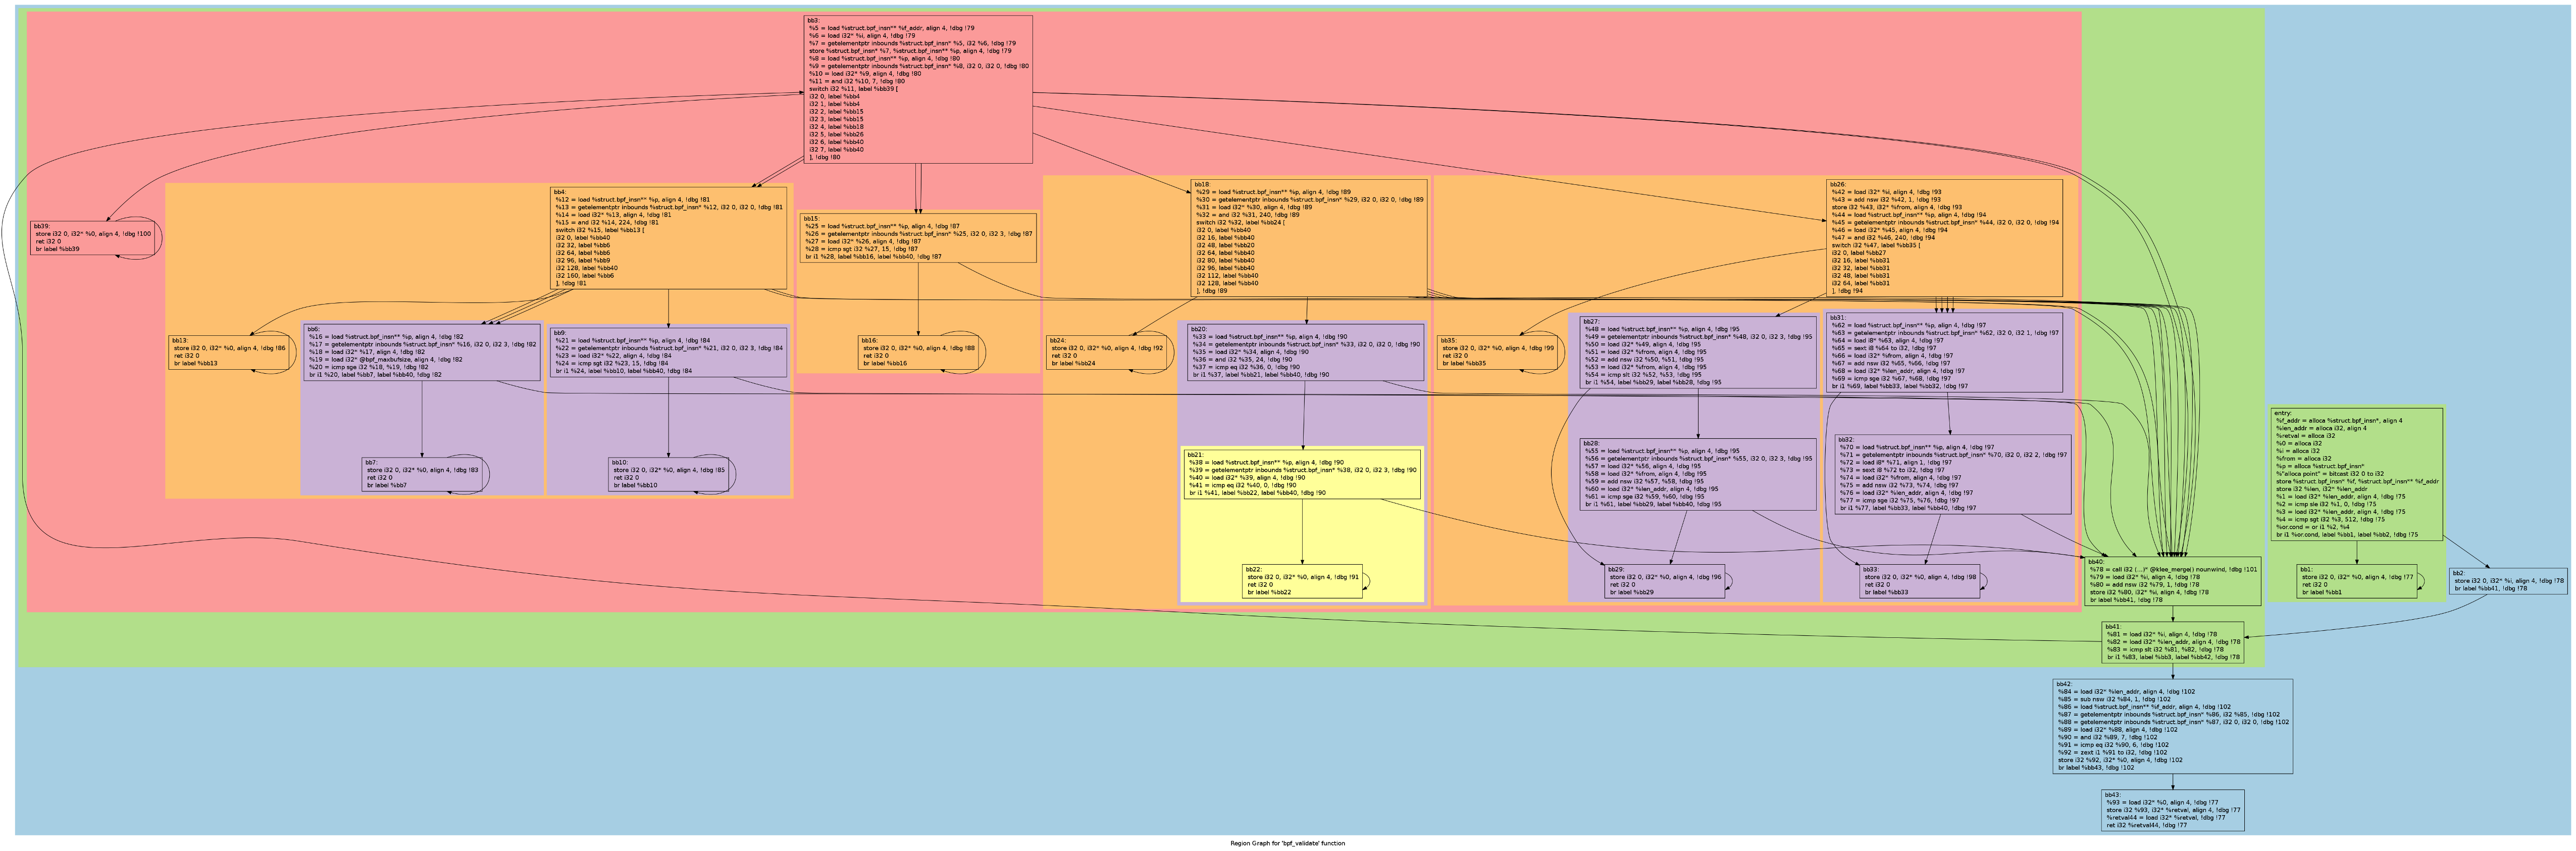
\includegraphics[width=\textwidth]{reg.png}
  \caption{Region information for bpf\_validate overlaid on the CFG. Each box is a \emph{basic block}; those in the same region are grouped by colour.}
\end{figure}

Internally, LLVM bitcode consists of \emph{basic blocks}, which are blocks of straigt-line code terminated by a control flow instruction. The control flow graph has basic blocks as nodes and directed edges representing control flow. We then group the basic blocks into \emph{Regions}. A Region \cite{regions} is a connected subgraph of a control flow graph that has exactly two connections to the remaining graph; regions may be nested. For instance, the body of an if statement or a while loop is a region.

In our algorithm, we track the regions an execution state is in. Whenever an execution path leaves a region $R$, it pauses and waits for other states in $R$ to leave $R$. Then, it tries to merge with other states paused at the same point before continuing. 

Any merging algorithms will crucially rely on pausing execution states at some point, because otherwise a state will be executed too far past the merge point and a chance to merge will be missed. A flawed algorithm might end up in a deadlock situation where the paused state never gets unpaused. However this cannot happen to ours as we only paused when there are some states in the region we left.

\subsubsection{When do we want to merge?}
We discovered experimentally that if we always merge execution states whenever possible, \klee takes a much longer time to solve the resulting constraints, outweighing the speedups offered by merging. Hence, we only merge two execution states if they are similar enough. We use two metrics for similarity: the number of memory addresses two states differ by as well as the number of constraints they have in common. We experiment with varying the threshold for these metrics in \S\ref{evaluation}.

While we may not want to merge two states at a certain merge point, we may wish to merge them at a later point. Our algorithm will automatically ensure that when one of two states that did not merge at a certain merge point reach another merge point, it waits for the other state to attempt to merge again.

\subsection{Simplify}
Whenever an execution state is modified (i.e. during merging and splitting), \klee must read the constraints on it and sometimes solve it. However as the execution state progresses through the control flow of the program, it adds more constraints; the problem is worsened when constraints are merged as two large expression trees are simply joined together. The simplify algorithm is an optimization that avoids this by simplifying the constraints and makes the solver queries easier and the expressions easier to store in \klee. This is particularly useful as often, constraints that arise from merging "cancel out" (simplify to true).

The first part of our simplifier uses a principle that we developed ourselves:
Consider an expression $E = A\cap(B\cup A)$. We consider cases: if $A$ were false, then E will be false regardless of the value of $(B\cup A)$. If $A$ were true, we can replaces occurences of $A$ in the RHS $(B\cup A)$ with true. Thus we can always replace occurences of $A$ in the RHS with true. The tree will then simplify to $A\cap(B\cup \text{True}) = A$. By duality, in $A\cup(B\cup A)$ we can replace occurances of $A$ in $(B\cup A)$ by false.

In the second part of the simplifier algorithm, we use simple theorems for simplification (eg. $A\cup \text{True} = \text{True}$) to complete the simplification. The simplifier algorithm will be repeatedly run until the expression does not change. This algorithm is fast and well-suited for the constraints produced by merging (with many AND's and OR's) that \klee did not simplify.

\section{Evaluation}\label{evaluation}
\setlength{\extrarowheight}{2ex}
\begin{table}
\begin{tabular}{|m{5.5cm} *{4}{| m{1.9cm} }|}
\hline
Name & LOC & Size(bytes) & \multicolumn{2}{p{3.4cm}|}{Time Taken(s)}\\ \cline{4-5}
 & & & \multicolumn{1}{p{1.7cm}|}{\klee} & \multicolumn{1}{p{1.7cm}|}{\leek}\\ \hline
bpf/bpf\_validate   &     154       &       100     &       254.625     &     6.258\\ \hline
netbsd/glob2        &     55        &       40      &       1.842       &      0.586\\ \hline
apache/get\_tag     &     114       &       10      &       66.164      &     62.467\\ \hline
mult\cite{statejoin}&     16        &       1       &       7.264       &     0.111\\ \hline
atol                &     50        &       12      &       7.790       &     18.035\\ \hline
edbrowse/ftpls      &     87        &       32      &       91.369      &     13.937\\ \hline
tr/expand           &     38        &       5       &       42.555      &     51.749\\ \hline
\end{tabular}
\caption{Time taken for \klee and \leek for various programs. 'Name' identifies the program as well as function we tested. 'LOC' is the lines of code as reported by David A. Wheeler's 'SLOCCount'. 'Size' is the size of the symbolic input.}
\label{tab:mainresult}
\end{table}

We evaluated \leek by selecting 7 benchmarks that were used in the literature before \cite{statejoin}\cite{zitser}\cite{klee}. We then ran both \leek and \klee on them, recording the time it took for both to symbolically execute each program. We used the same merging threshold for all of them. The results are presented in Table \ref{tab:mainresult}. \leek performs better than \klee on 5 out of 7 of these programs. Over all the programs, the mean improvement is 1687\% and the median improvement is 314\%. Note that the results \emph{underestimate} the improvements that \leek provides as the merging threshold is not optimal for all of them; for instance \leek's runtime on ftpls can be further reduced to 0.186s with optimum settings.

Upon examining our results, we program structures that greatly affected the improvement. Select statements were highly amenable to merging as differenc cases are are ofter handled similarly. Another area is loops; \klee spends most of its time analyzing loops because they spawn many execution states. Such loops typically advance a loop counter (an integer or pointer) and do so either once per iteration or multiple times per iteration. When the counter is advanced once per iteration, the execution states spawned in one iteration can easily be merged because the loop counter is the same; however this is not true if the amount of advancement is loop-dependent.

While our algorithm has such a limitation, advancing the counter a variable number of times leads to more dangerous code, as we could more easily go out of bounds. Even so we believe there is nothing fundamentally very different about these two types of loops and future work is aimed at speeding up analysis of such loops.


\begin{figure}
  \hfill
  \begin{minipage}[t]{.45\textwidth}
    \begin{center}  
      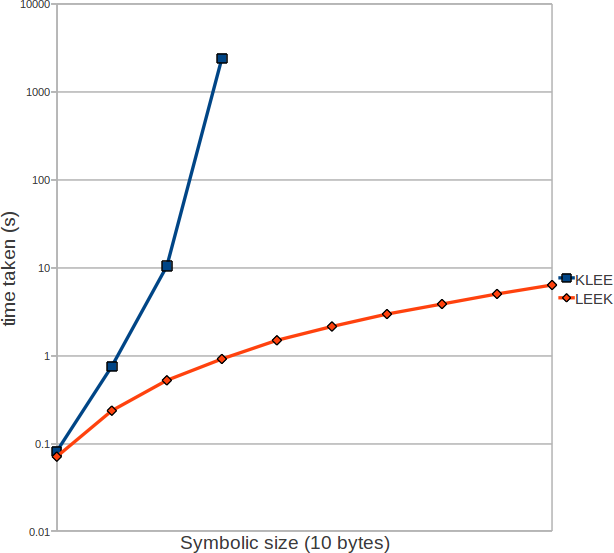
\includegraphics[width=\textwidth]{bpf_graph.png}
      \caption{Time taken for analysis versus size of symbolic input. Note that the time taken is plotted on a log scale in order to compare the two lines.}
      \label{bpfgraph}
    \end{center}
  \end{minipage}
  \hfill
  \begin{minipage}[t]{.45\textwidth}
    \begin{center}  
      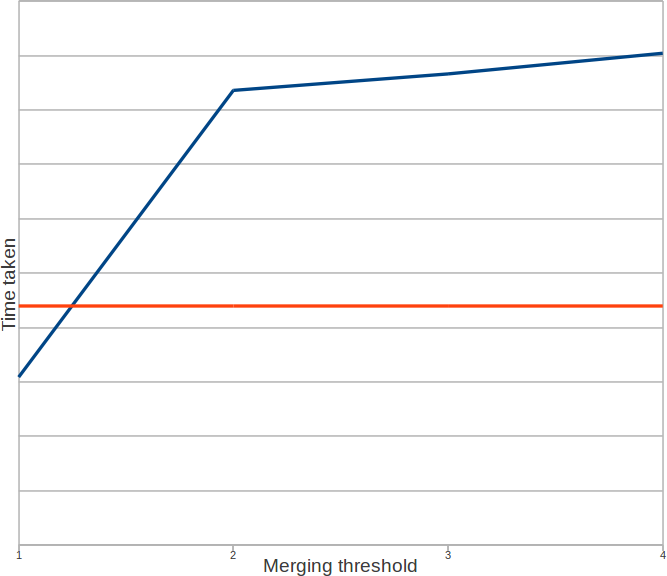
\includegraphics[width=\textwidth]{threshold_graph.png}
      \caption{Time taken for analysis versus merging threshold. The flat line is the time it takes for \klee to analyze the program.}
      \label{threshgraph}
    \end{center}
  \end{minipage}
  \hfill
\end{figure}

Furthermore, we performed two other small experiments. Firstly, we measured time taken to analyze a program as a function on the number of bytes made symbolic for both \klee and \leek to test the hypothesis that \leek can reduce the asymptotic time needed to symbolically execute certain programs. We chose bpf\_validate for this. The results are shown in figure \ref{bpfgraph}. Clearly, \klee's execution time is super-exponential in the symbolic input size while \leek's is sub-exponential.

We also explored varying the parameters for the merging threshold. We found that changing threshold based on the number of constraints had a much smaller effect compared to changing the threshold based on the number of memory addresses (variables) changed. Hence we only plot the later in figure \ref{threshgraph}. The optimum threshold is clearly 0, ie we only merge if \emph{no} memory addresses have changed.

\section{Related work}\label{related}
There have been two main approaches to the problem of program verification: static analysis \cite{MC} and dynamic analysis. Static analysis checks the program without running it, ie, only by looking at the source code. Such analysis often suffers from high false positives due to the fact that they are not precise enough; in particular most of them are path-insensitive. This means that they could potentially report an error that will occur on some execution path through a program even if that path is not feasible. Adding path sensitivity to static analysis is inappropriate as they are designed to be lightweight analyses and checking the feasibility of paths would require some sort of heavyweight decision procedures.

Dynamic analysis, on the other hand, monitors programs as they are run and report only errors that actually occur; thus they never report false positives. An example that is commonly used is Valgrind \cite{valgrind}, a framework that automatically reports memory management bugs (such as reading / writing out of bounds) and concurrency bugs (such as race conditions or deadlocks). However these tools only report errors that occur in given concrete runs; thus, someone has to supply test cases to them.

Symbolic analysis combines the advantages of both approaches; it only needs the source code of a program to work and it also never reports false positives. Furthermore, it is much more scalable and less labour-intensive than formal verification methods like model checking and theorem proving. Symbolic analysis was first proposed in 1976 \cite{old}, but practical symbolic execution tools have only emerged recently \cite{klee}\cite{dart}. This is because only recently do we have powerful decision procedures \cite{bitvecarray} for properties we care about, programs that can decide, for instance, if a certain execution path is feasible. Although the problem is NP-hard (all the decision procedures use a SAT solver, and 3-SAT is the canonical NP-hard problem) in general, heuristics for decision procedures have been proven to be fast enough; for instance, fast heuristic algorithms for linear integer constraints that can accurately model the modular arithmetic used by computers exist.

Symbolic analysis suffers from the path explosion problem, the problem that even though the number of feasible paths through a program is much less than the number of inputs, it is still too large. Most research has gone into using better heuristics to explore the search space; for instance, \klee proritizes execution states that will explore more code, while AEG \cite{aeg} aims to explore only those states that are likely to lead to buffer overflows (mainly, the symbolic input is as long as possible). Other approaches are pruning redundant states \cite{rwset}, which can be viewed as a special case of merging, as well as performing analysis compositionally by re-using function summaries \cite{cdtg}. \cite{loopsum} explores modeling linear constraints on loop iterations. CUTE \cite{cute} investigates \emph{concolic execution}, where concrete runs are used to guide the symbolic execution.

State merging has previously been explored by Hansen et. al. \cite{statejoin} for symbolically executing binaries. However, we believe that an analysis such as this is much better suited to targeting a higher-level language such as LLVM bitcode as calculating the control flow structure of programs without the source code is not easy; one needs to use a disassembler and even then, the whole CFG may not be calculated. Also, Hansen et. al. did not show that state merging could be used on real-life examples and not just toy programs, wheares we have.

\section{Conclusions}\label{conclusions}
We have successfully implemented an algorithm for the merging of states for the execution of \klee, which is initally not well-developed. Our results show a clear change of the time required to analyze the program between \klee and \leek, which is from exponential to sub-exponential respectively. The median speed-up of 317\% ascertains our hypothesis that a merging algorithm outperforms a non-merging one, while our other experiments confirm the rest of the hypotheses.

We should first explain that our algorithm and many others are created to replicate the logical processes in the human mind. If a human would analyze BPF, he would be able to tell where redundancies occur and process only the relevant lines of code. This pattern recognition system and logical reasoning of the brain is what our code aims to attain.

As such, rather than just an algorithm for \klee we have demonstrated logical reasoning within the processes that goes into merging that, as of now, is not well developed. This reasoning within merging has the potential to be used in any analysis programs that may tackle recursion or iteration that are commonly seen in programming. In other words, other algorithms can be designed around the ideas that originally created our algorithm.

Our algorithm can still be greatly improved to discover more potential merge points as well as to use better heuristics for when to merge. For example our wait-and-merge algorithm as described in \S 3.2 cannot compare to the human instinct, which (in our experience) can quickly determine which execution states are similar. We also should consider to extend the merge algorithm to cater to the messy \emph{goto} statements which prevent regions from being created. 

\section{Appendix}

\subsection{Correctness}
The merge operation is a function that takes two execution states and returns a single one. An execution state comprises of a set of constraints that hold on its input as well as a set of mappings from memory locations to symbolic expressions representing the heap and stack of a running program.

Given an execution state $E_1$ with constraints $C_1$ and a mapping $M_1$ such that $M_1 = M_1(loc_i)$ (a function that goes from the $i^{th}$ location in memory to an expression and an execution state $E_2$ with constraints $C_2$ and a mapping $M_2$, the merged state $E_m$ will have constraint $C_m = C_1 \vee C_2$ with a mapping $M_m(loc_i) = ITE(C_1, M_1(loc_i), M_2(loc_i))$. The $ITE$ (\emph{if-then-else}) function returns its second argument if its first argument is true, otherwise it returns its third argument.

We prove here that our algorithm is sound and complete with respect to the base \klee system. Roughly, soundness means that all reported errors are acutal errors and completeness means that all errors are reported. We show that for a given program $P$, \leek will report an error for a certain input $I$ iif \klee reports an error for $I$. Note that our system is only sound and complete with respect to \klee; \leek is only sound and complete when klee is too. For instance, \klee does not support symbolic floating point; thus if it does not catch a certain input neither will \leek.

As \klee operates, it generates (by branching) and destroys (by terminating) execution states; \leek additionally merges execution states. The key invariant $T$ that always holds on the execution states is this: $T$ means that every concrete execution of $P$ satisfies the constraints of exactly one execution state, including states that are active and states that have been terminated, and every execution state is reachable by some concrete execution of $P$.

How does this invariant imply soundness and completeness of \leek if \klee is sound and complete? Since the input $I$ will satisfy one execution state, when all the states terminate, there must exist some terminated state which $I$ satisfies; we can then rely on the completeness of \klee to ensure that that state will generate an error report. Also if a state generates an error report, we know by the second part of the invariant there is some input that satisfies the state and hence by the soundness of klee that it is an input that generates unwanted behaviour.

This invariant clearly holds at the start, when \emph{all} executions satisfy the only execution state, which has no constraints. When forking execution states, say on a condition $c$, klee will fork execution like so: $\{E\} \rightarrow \{E_T, E_F\}$, replacing $E$ with $E_T$ and $E_F$, and if $E$ had constraints $C$, $E_T$ has constraints $C \wedge c$ and $E_F$ has constraints $C \wedge \neg c$. If $I$ satisfied $C$, the invariant still holds as $I$ satisfies exactly one of $E_T$ and $E_F$ (since $E_T \vee E_F$ = true and $E_F \wedge E_T$ = false). Terminating states also mantain the invariant as it merely changes a state from active to terminated.

What merging does is this: $\{E_1, E_2\} \rightarrow \{E_m\}$, replacing $E_1$ and $E_2$ with $E_m$. If $E_1$ had constraints $C_1$ and $E_2$ had $C_2$, then $E_M$ has constraints $C_1 \vee C_2$. If $I$ satisfied one of $C_1$ or $C_2$, it satisfies $E_m$ as $C_1 \vee C_2$ is true when one of $C_1$ and $C_2$ is true. If it did not satisfy one of $C_1$ or $C_2$, it does not satisfy $C_1 \vee C_2$ as $F \vee F = F$.

\begin{thebibliography}{9}
\bibitem{old}
         J. C. King.
         Symbolic execution and program testing.
         In \emph{Communications of the ACM, 1976}.

\bibitem{klee}
         D. Dunbar, C. Cadar, D. Engler. 
         KLEE: Unassisted and Automatic Generation of High-Coverage Tests for Complex Systems Programs.
         In \emph{Operating Systems Development and Implementation (OSDI 2008)}

\bibitem{exe}
          C. Cadar, V. Ganesh, P.M. Pawlowski, D.L. Dill, D.R. Engler
          EXE: Automatically Generating Inputs of Death.
      	  In\emph{ Proceedings of the 13th ACM Conference on Computer and Communications Security (CCS 2007)}
         
\bibitem{dart}
          P. Godefroid, N. Klarlund, K. Sen. 
          DART: Directed Automated Random Testing.
          In\emph{ Proceedings of the 2005 ACM SIGPLAN conference on Programming language design and implementation (PLDI 2005)}
	
\bibitem{loopsum}
        D. Kroening, N. Sharygina, S. Tonetta, A. Tsitovich, C. M. Wintersteiger.
        Loop Summarizationusing Abstract Transformers.
        In\emph{ 6th International Symposium on Automated Technology for Verification and Analysis (ATVA 2008)}

\bibitem{cdtg}
        P. Godefroid.
        Compositional Dynamic Test Generation.
        In\emph{ Proceedings of the 34th annual ACM SIGPLAN-SIGACT symposium on Principles of programming languages (POPL 2007)}
        
\bibitem{regions}
        R. Johnson, D. Pearson, K. Pingali.
        The Program Structure Tree: Computing Control Regions in Linear Time.
        In\emph{ Programming Languages Implementation and Design (PLDI 1994)}

\bibitem{rwset}
        P. Boonstoppel, C. Cadar, D. Engler.
        RWset: attacking path explosion in constraint-based test generation.
        In\emph{ International Conference on Tools and Algorithms for the Constructions and Analysis of Systems (TACAS 2008)}
        
\bibitem{bitvecarray}
        V. Dill.
        A decision procedure for bitvectors and arrays.
        In\emph{ Computer Aided Verification, 2007}
        
\bibitem{statejoin}
        T. Hansen, P. Schachte, H. Søndergaard.
        State Joining and Splitting for the Symbolic Execution of Binaries.
        In\emph{ Lecture Notes in Computer Science, 2009, Volume 5779/2009.}
        
\bibitem{valgrind}
        N. Nethercote, J. Seward.
        Valgrind: a framework for heavyweight dynamic binary instrumentation.
        In\emph{ Proceedings of the 2007 ACM SIGPLAN conference on Programming language design and implementation (PLDI 2007)}
        
\bibitem{modelchecking}
        E.M. Clarke.
        Model Checking.
        In\emph{ Foundations of Software Technology and Theoretical Computer Science, 1997}
        
\bibitem{aeg}
        T. Avgerinos, S. K. Cha, B. Lim T. H. and D. Brumley.
        AEG: Automatic Exploit Generation.
        In\emph{ Network and Distributed System Security Symposium (NDSS 2011)}

\bibitem{awft}
        P. Godefroid, M.Y. Levin, D. Molnar.
        Automated Whitebox Fuzz Testing.
        In\emph{ Network and Distributed System Security Symposium (NDSS 2007)}
        
\bibitem{dtg}
        R. Majumdar, R.G. Xu.
        Directed test generation using symbolic grammars.        
        In \emph{ASE '07 Proceedings of the twenty-second IEEE/ACM international conference on Automated software engineering}
       
\bibitem{cute}        
        K. Sen, D. Marinov, G. Agha. 
        CUTE: A Concolic Unit Testing Engine for C. 
        In\emph{ 5th joint meeting of the European Software Engineering Conference and ACM SIGSOFT Symposium on the Foundations of Software Engineering (ESEC/FSE'05)}

\bibitem{MC}
        S. Hallem, B. Chelf, Y. Xie, and D. Engler.
        A System and Language for Building System-Specific, Static Analyses.
        In\emph{ Proceedings of the ACM SIGPLAN 2002 Conference on Programming Language Design and Implementation (PLDI 2002)}

\bibitem{zitser}
        Zitser M., Lippmann R., Leek T. 
        Testing Static Analysis Tools Using Exploitable Buffer Overflows From Open Source Code.
        In \emph{ACM SIGSOFT Symposium on the Foundations of Software Engineering (FSE 2004)}

\end{thebibliography}



\end{document}
